\documentclass[a4paper,12pt]{article}
\usepackage[russian]{babel}

% Самые необходимые пакеты
\usepackage[T2A]{fontenc}
\usepackage[utf8]{inputenc}
\usepackage[russian]{babel}
\usepackage{geometry}
\usepackage{amsmath}
\usepackage{graphicx}
\usepackage{float} 
\usepackage{xcolor}
\usepackage{listings}
\usepackage{hyperref}
\usepackage{array}
\usepackage{caption}
\usepackage{booktabs}
\usepackage{amssymb}
\usepackage{subcaption}
\usepackage{caption}
\captionsetup[figure]{name=Рисунок}
\captionsetup[table]{name=Таблица}
\usepackage{pgfplots}
\pgfplotsset{compat=1.18}
\usetikzlibrary{arrows.meta}
\usepackage{capt-of}
\usepackage{multirow}


\lstset{
	language=Matlab,
	basicstyle=\ttfamily\small,
	keywordstyle=\color{blue}\bfseries,
	commentstyle=\color{gray}\itshape,
	stringstyle=\color{red},
	numberstyle=\tiny\color{gray},
	numbers=left,
	stepnumber=1,
	numbersep=8pt,
	backgroundcolor=\color{white},
	frame=single,
	breaklines=true,
	breakatwhitespace=true,
	tabsize=4,
	showspaces=false,
	showstringspaces=false,
	captionpos=b,
	escapeinside={\%*}{*)},
}
\geometry{left=1.5cm, right=2cm, bottom=2cm, top=2cm}

\begin{document}
	
	% Титульный лист
	\begin{titlepage}
		\centering
		\vspace*{1cm}
		
		% Министерство
		{\small
			Министерство науки и высшего образования Российской Федерации\\
			Федеральное государственное автономное образовательное учреждение\\
			высшего образования\\
			«Национальный исследовательский университет ИТМО»\\
		}
		
		\vspace{2cm}
		
		% Факультет
		{\large
			Факультет систем управления и робототехники\\
		}
		
		\vspace{3cm}
		
		% Основной заголовок
		{\Huge\bfseries
			ОТЧЕТ\\
		}
		\vspace{0.5cm}
		{\LARGE\bfseries
			о лабораторной работе №1\\
		}
		
		\vspace{1cm}
		
		% Дисциплина и тема
		{\Large
			По дисциплине: «Электронные устройства систем управления»\\
			\vspace{0.5cm}
			Тема: «Операционный усилитель в основных схемах включения»\\
			\vspace{0.5cm}
			Вариант: 6
		}
		
		\vspace{3cm}
		
		% Информация о студенте и преподавателях
		\begin{minipage}{0.4\textwidth}
			\raggedright
			{\large
				Студенты:\\
			}
			Охрименко Е. \\
			Шишкина М. \\
			Чупрова Д. \\
		\end{minipage}
		\hfill
		\begin{minipage}{0.4\textwidth}
			\raggedleft
			{\large
				Преподаватели:\\
			}
			Власов С. М. \\
			Зарина О. А.
		\end{minipage}
		
		\vfill
		
		% Город и год
		{\large
			Санкт-Петербург\\
			2026\\
		}
		
	\end{titlepage}
	
	\newpage
	\tableofcontents
	
	\newpage
	\section{Исследование дифференциального усилителя}
	
	В соответствии с заданием в качестве резистора обратной связи выберем резистор номиналом:
	\[
	R_2 = 10~\text{кОм}.
	\]
	
	Выходное напряжение дифференциального усилителя определим по формуле:
	\[
	U_{\text{вых}} =
	\frac{R_2}{R_1}
	\left(
	U_2 - U_1
	\right)
	\]
	
	По варианту задания коэффициент усиления \(K = 10\), значит должно быть выполнено соотношение: 
	\[
	\frac{R_2}{R_1} = \frac{R_4}{R_3} = K = 10
	\]
	
	
	Так как:
	\[
	R_2 = 10~\text{кОм}
	\]
	Можно посчитать сопротивление резистора \(R_1\):
	\[
	R_1 = \frac{R_2}{K}
	= \frac{10~\text{кОм}}{10}
	= 1~\text{кОм}.
	\]
	
	Для выполнения условия симметрии:
	\[
	\frac{R_4}{R_3} = \frac{R_2}{R_1} = 10,
	\]
	Выбираем:
	\[
	R_3 = 1~\text{кОм} \quad
	R_4 = 10~\text{кОм}
	\]
	
	Таким образом, окончательно получаем:
	\[
	R_1 = 1~\text{кОм}, \quad
	R_2 = 10~\text{кОм}, \quad
	R_3 = 1~\text{кОм}, \quad
	R_4 = 10~\text{кОм}.
	\]
	
	Итоговые значения:
	\[
	U_{\text{вых}} = 10\,(U_2 - U_1).
	\]
	
	Соберем схему дифференциального усилителя и подставим соответствующие значения резисторов.
	
	
	\begin{figure}[H]
		\centering
		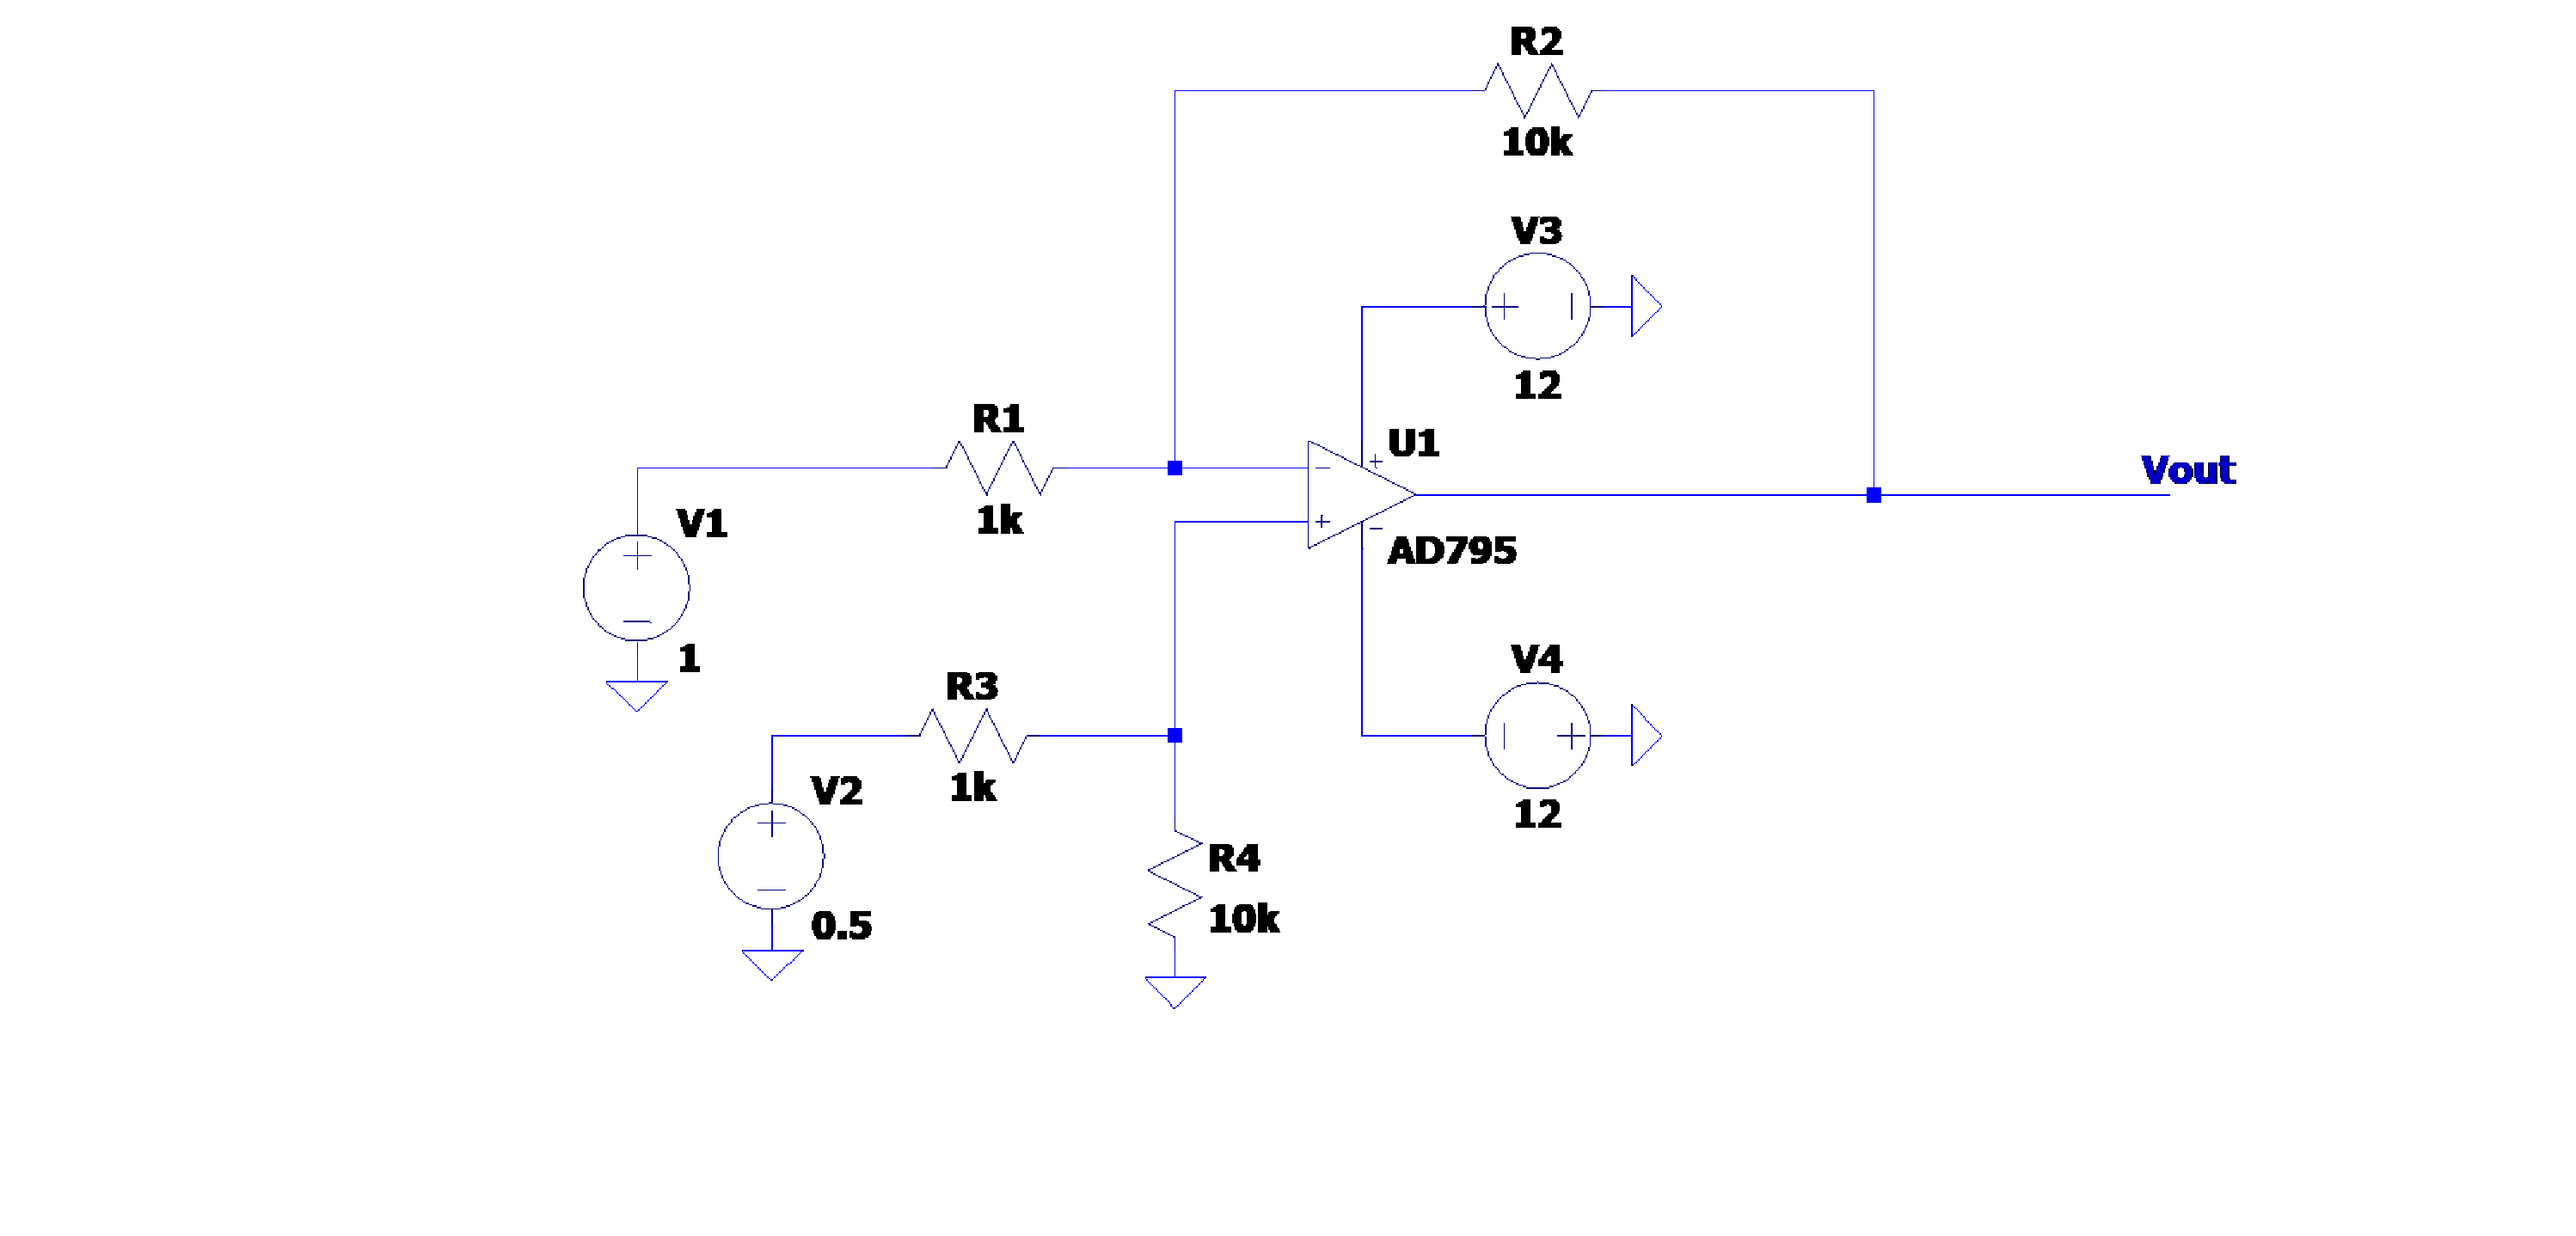
\includegraphics[width=1\textwidth]{../images/task1/1.1/diff_amplifier.pdf}
		\caption{Дифференциальный усилитель}
	\end{figure}
	
	Теперь измерим значения \(U_{\text{вых}}\) для различных пар \(U_1\) и \(U_2\), соотнесем экспериментально полученные данные с данными, посчитанными по формуле. Результаты измерения приведены в таблице~\ref{tab:diff_results}.

	\begin{table}[H]
		\centering
		\caption{Сравнение расчётных и моделируемых значений выходного напряжения
			дифференциального усилителя}
			\label{tab:diff_results}
		\begin{tabular}{c c c c c c}
			\toprule
			№ & $U_1$, В & $U_2$, В & $U_{\text{вых}}^{\text{мод}}$, В &
			$U_{\text{вых}}^{\text{расч}}$, В & $\Delta U$, В \\
			\midrule
			1 & 1    & 0.5  & -4.99 & -5.0  & 0.01 \\
			2 & 0.5  & 1    &  4.99 &  5.0  & 0.01 \\
			3 & 0.2  & 0.8  &  5.99 &  6.0  & 0.01 \\
			4 & 0.8  & 0.2  & -5.99 & -6.0  & 0.01 \\
			5 & -0.5 & 0.5  &  9.2 & 10.0  & 0.8 \\
			6 & 0.5  & -0.5 & -9.2 & -10.0 & 0.8 \\
			\bottomrule
		\end{tabular}
	\end{table}
	
	Экспериментально измеренные значения выходного напряжения в целом совпали с
	расчётными по формуле $U_{\text{вых}} = 10(U_2 - U_1)$. При небольших входных
	напряжениях расхождение оказалось минимальным.
	
	\subsection{Исследование влияния синфазной и противофазной помехи}
	
	Соберем схему дифференциального усилителя при имитации воздействия помехи. 
	
	\begin{figure}[H]
		\centering
		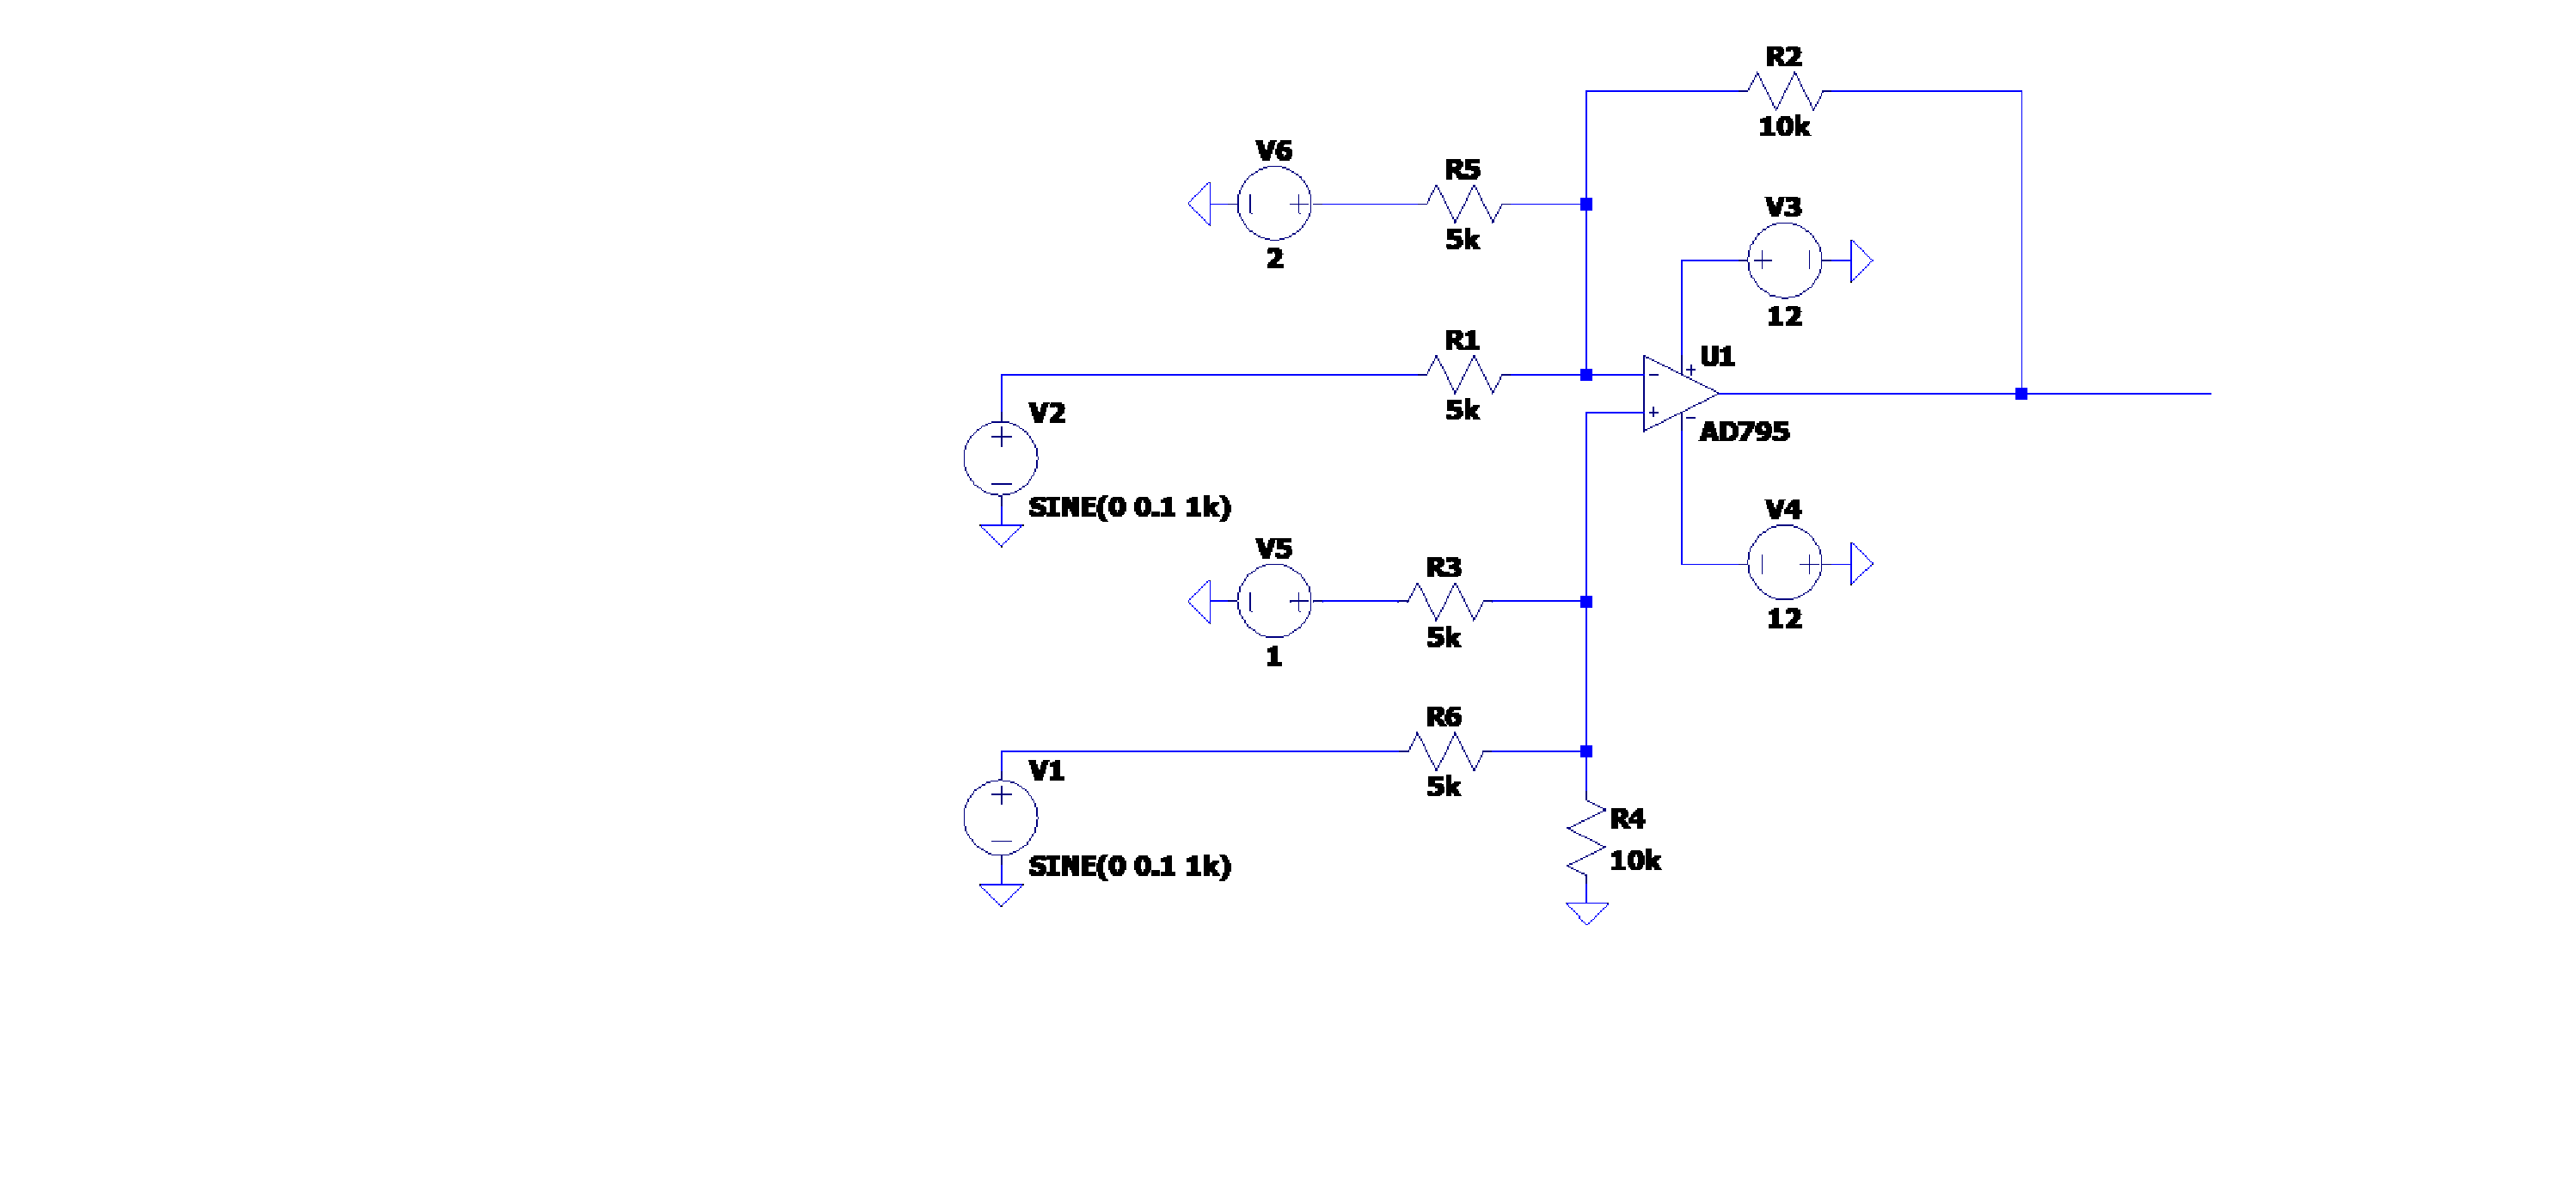
\includegraphics[width=1\textwidth]{../images/task1/1.2/diff_amplifier_interference.pdf}
		\caption{Дифференциальный усилитель при имитации воздействия помехи}
	\end{figure}
	
	
	В первом случае одинаковый синусоидальный сигнал подавался одновременно
	на инвертирующий и неинвертирующий входы (синфазная помеха). 	
	
	\begin{figure}[H]
		\centering
		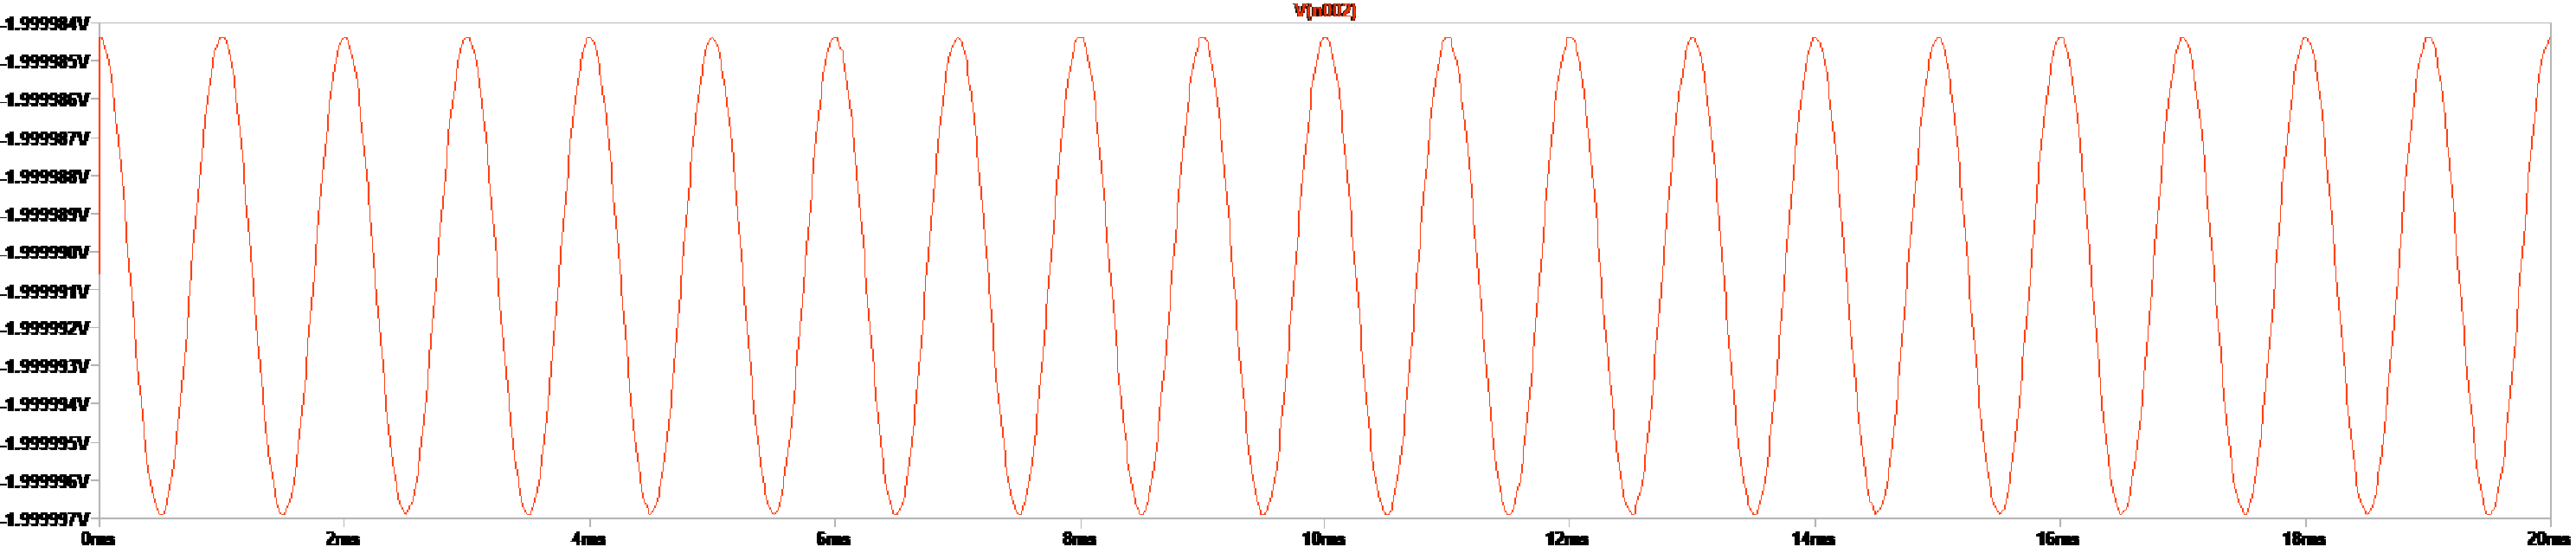
\includegraphics[width=1\textwidth]{../images/task1/1.2/common-mode_interference.pdf}
		\caption{Имитация воздействия синфазной помехи}
	\end{figure}
	
	Во втором
	случае сигнал подавался только на один вход, что имитирует разностное
	воздействие.
	
	
	\begin{figure}[H]
		\centering
		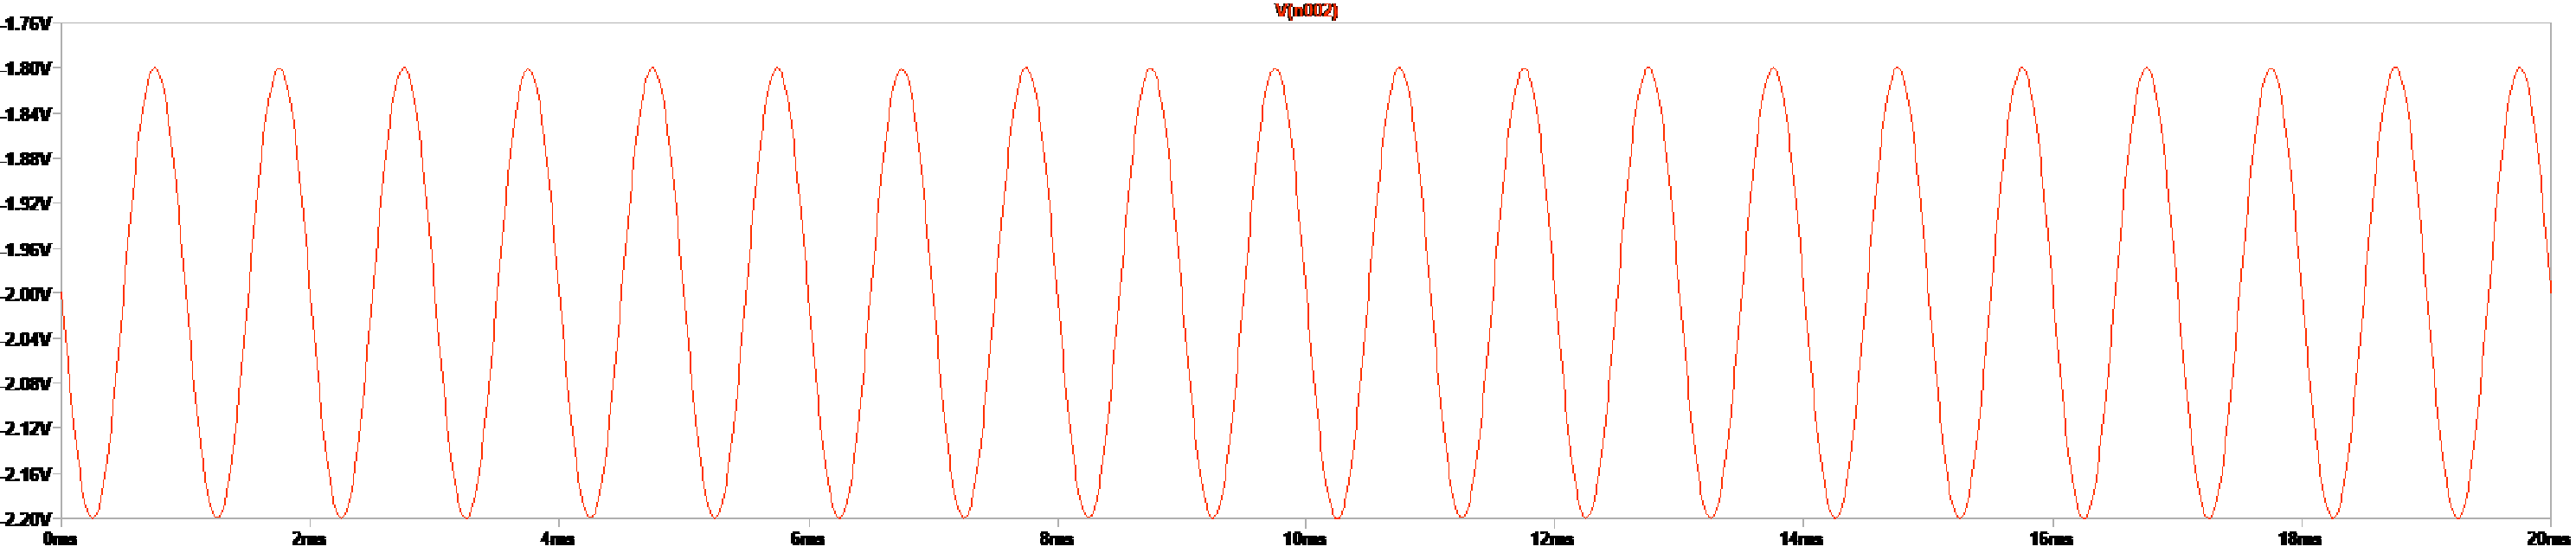
\includegraphics[width=1\textwidth]{../images/task1/1.2/pro-phase_interference.pdf}
		\caption{Имитация воздействия противофазной помехи}
	\end{figure}
	
	При подаче одинакового гармонического сигнала на оба входа
	наблюдается значительное подавление помехи на выходе.
	
	При подаче сигнала только на один вход на выходе появляется
	усиленный синусоидальный сигнал.
	
	
	
	
	
	\newpage
	\section{Исследование ОУ в режиме суммирования постоянных сигналов}
	
	\subsection{Инвертирующий сумматор}
	
	Соберем схему инвертирующего сумматора на операционном усилителе. 
	
		\begin{figure}[H]
		\centering
		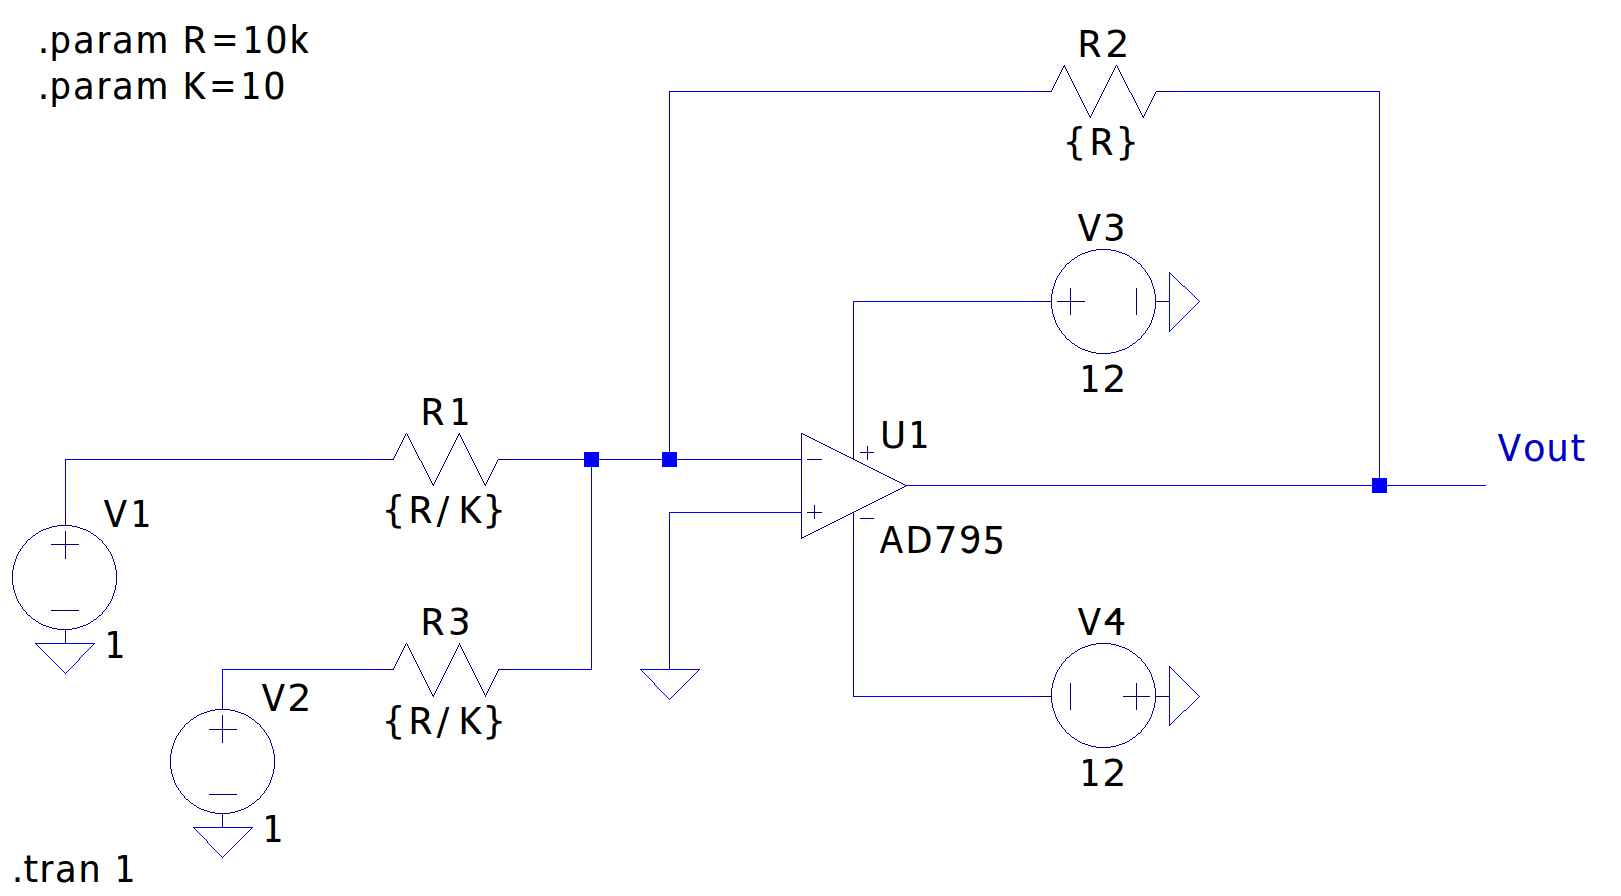
\includegraphics[width=1\textwidth]{../images/task2/2.1/t1.png}
		\caption{Инвертирующий сумматор на ОУ}
	\end{figure}
	
	Выходное напряжение инвертирующего сумматора определяется выражением:
	\[
	U_{\text{вых}} = -\left(\frac{R_2}{R_1}U_1 + \frac{R_2}{R_3}U_2\right)
	\]
	
	По схеме заданы параметры:
	\[
	R_2 = R \quad R_1 = \frac{R}{k}\quad R_3 = \frac{R}{k}
	\]
	\[
	R = 10\,\text{кОм} \quad k = 10
	\]
	
	Подставим значения в формулу:
	\[
	U_{\text{вых}} =
	-\left(
	\frac{R}{R/k}U_1 +
	\frac{R}{R/k}U_2
	\right) = -(kU_1 + kU_2)
	\]

	При \(k=10\):
	\[
	U_{\text{вых}} = -10(U_1 + U_2)
	\]
	
	Теперь измерим значения \(U_{\text{вых}}\) для различных пар \(U_1\) и \(U_2\), соотнесем экспериментально полученные данные с данными, посчитанными по формуле. Результаты измерения приведены в таблице~\ref{tab:sum_results}.
	
	\begin{table}[H]
		\centering
		\caption{Сравнение расчётных и моделируемых значений выходного напряжения инвертирующего сумматора}
		\label{tab:sum_results}
		\begin{tabular}{c c c c c c}
			\toprule
			№ & $U_1$, В & $U_2$, В & $U_{\text{вых}}^{\text{мод}}$, В &
			$U_{\text{вых}}^{\text{расч}}$, В & $\Delta U$, В \\
			\midrule
			1 & 0.2  & 0.3  & -4.9 & -5.0 & 0.1 \\
			2 & 0.4  & 0.4  & -7.9 & -8.0 & 0.1 \\
			3 & 0.1  & 0.5  & -5.9 & -6.0 & 0.1 \\
			4 & 0.7  & 0.2  & -8.9 & -9.0 & 0.1 \\
			5 & -0.3 & 0.2  &  0.9 &  1.0 & 0.1 \\
			6 & 0.3  & -0.6 &  2.9 &  3.0 & 0.1 \\
			\bottomrule
		\end{tabular}
	\end{table}
	
	Из таблицы видно, что рассчитанные значения выходного напряжения хорошо
	совпадают с результатами моделирования. Различие не превышает 0.1 В и
	связано с тем, что операционный усилитель в модели является неидеальным.
	
	Полученные данные подтверждают, что схема работает как инвертирующий
	сумматор и описывается выражением
	\[
	U_{\text{вых}} = -10(U_1 + U_2).
	\]
	
	\subsection{Неинвертирующий сумматор}
	
		Соберем схему неинвертирующего сумматора на операционном усилителе. 
	
	\begin{figure}[H]
		\centering
		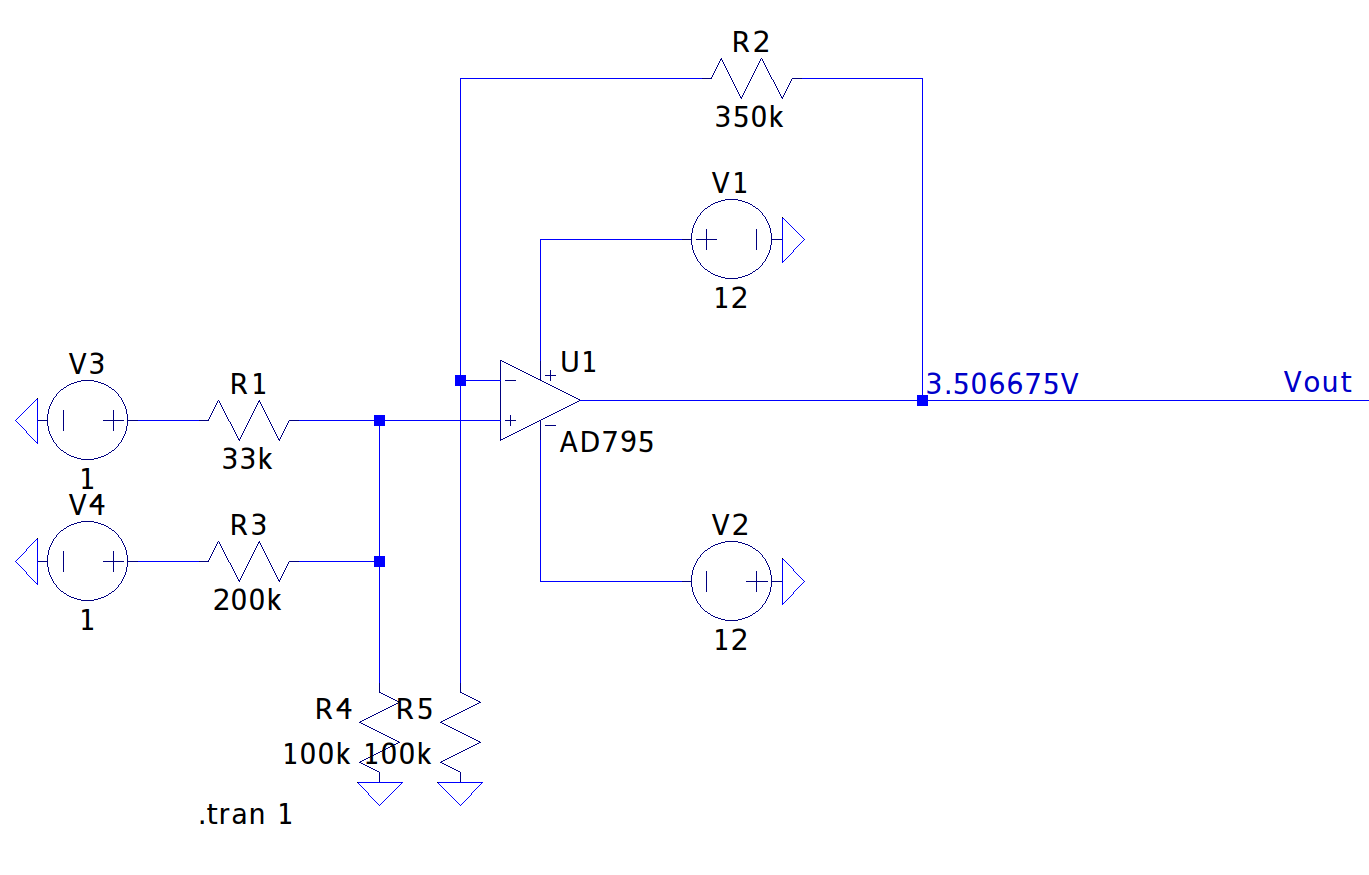
\includegraphics[width=1\textwidth]{../images/task2/2.2/t2.png}
		\caption{Неинвертирующий сумматор на ОУ}
	\end{figure}
	
	Воспользуемся коэффициентами для нашего варианта:
	\[
	K_1 = 3, \qquad K_2 = 0.5
	\]
	
	Из методички зафиксируем значения для резисторов:
	\[
	R_4 = R_5 = 100~\text{кОм}
	\]
	
	Выходное напряжение определяется выражением:
	\[
	U_{\text{вых}} = \frac{R_5}{R_1}U_1 + \frac{R_5}{R_3}U_2
	= K_1 U_1 + K_2 U_2
	\quad \Longrightarrow \quad
	K_1 = \frac{R_5}{R_1}
	\qquad
	K_2 = \frac{R_5}{R_3}
	\]
	
	Подставим $R_5 = 100~\text{кОм}$:
	
	\[
	R_1 = \frac{100}{3} \approx 33~\text{кОм}
	\]
	\[
	R_3 = \frac{100}{0.5} = 200~\text{кОм}
	\]
	
	Резистор обратной связи определяется из условия:
	\[
	\frac{R_2}{R_4} =
	\frac{R_5}{R_1} +
	\frac{R_5}{R_3}
	\]
	
	\[
	\frac{R_2}{100} = 3 + 0.5 = 3.5
	\]
	
	\[
	R_2 = 350~\text{кОм}
	\]
	
	
	Теоретическое уравнение выходного напряжения:
	\[
	U_{\text{вых}} = 3U_1 + 0.5U_2
	\]

	Теперь измерим значения \(U_{\text{вых}}\) для различных пар \(U_1\) и \(U_2\), соотнесем экспериментально полученные данные с данными, посчитанными по формуле. Результаты измерения приведены в таблице~\ref{tab:noninv_sum_results}.

	
	\begin{table}[h]
		\centering
		\caption{Сравнение расчётных и моделируемых значений выходного напряжения неинвертирующего сумматора}
		\label{tab:noninv_sum_results}
		\begin{tabular}{c c c c c c}
			\toprule
			№ & $U_1$, В & $U_2$, В & $U_{\text{вых}}^{\text{мод}}$, В &
			$U_{\text{вых}}^{\text{расч}}$, В & $\Delta U$, В \\
			\midrule
			1 & 1  & 1  & 3.51 & 3.5 & 0.01 \\
			2 & 0.4  & 0.4  & 1.4 & 1.40 & 0.00 \\
			3 & 0.1  & 0.5  & 0.54 & 0.55 & 0.01 \\
			4 & 0.7  & 0.2  & 2.2 & 2.20 & 0.00 \\
			5 & -0.3 & 0.2  & -0.80 & -0.80 & 0.00 \\
			6 & 0.3  & -0.6 & 0.61 & 0.60 & 0.01 \\
			\bottomrule
		\end{tabular}
	\end{table}
	
	
	Как видно из таблицы~\ref{tab:noninv_sum_results}, моделируемые значения выходного напряжения хорошо совпадают с расчётными, полученными по формуле
	\[
	U_{\text{вых}} = 3U_1 + 0.5U_2
	\]
	
	
	\newpage
	\section{Вывод}
	
	В ходе работы мы изучили основные схемы включения операционного усилителя: дифференциальный усилитель, инвертирующий и неинвертирующий сумматоры.
	
	Мы рассчитали номиналы резисторов для каждого случая и собрали схемы в модели. Полученные значения выходного напряжения во всех экспериментах хорошо совпали с расчётными. Небольшие расхождения связаны с неидеальностью модели операционного усилителя и округлением номиналов.
	
	В результате мы убедились, что дифференциальный усилитель усиливает разность сигналов, а сумматоры выполняют сложение входных напряжений с заданными коэффициентами.
	
	

	Материалы работы: \href{https://github.com/decadeos/ITMO/tree/master/3_course/EDCS/lab1}{\texttt{github.com}}
	
\end{document}